% SPDX-FileCopyrightText: 2023 Iegor Riepin, Tom Brown
%
% SPDX-License-Identifier: CC-BY-4.0

\subsection{Signal 1: quality of local renewable resources}

Our first step is to isolate the signal associated with the difference in quality of local renewable resources. Consider a case when datacenters are located in Denmark, Germany, and Portugal (Figure \ref{fig:dashboard1}: panel a). There are three different types of renewable resources represented by the three sites, with Denmark having a good wind resource, Germany having a moderate wind and solar resources, and Portugal having a good solar resource. The quality of local renewable resources is reflected by the average annual capacity factor for onshore wind and solar PV, as shown in the panels b and c,

Figure \ref{fig:dashboard1}: panel d shows the modelled cost-optimal capacity of renewable generators and battery storage for 24/7 matching. In the case of inflexible loads, the procurement strategy must ensure a sufficient amount of carbon-free electricity is available round-the-clock \textit{at each site}. Due to the non-dispatchable nature of renewable resources and the relatively high energy costs of battery storage, the cost-optimal portfolio is much larger than the load. To cover the 100 MW load with perfect hourly matching, the consumer would have to procure combined wind and solar PV generators of approx. 900~MW in Denmark and 1300~MW in Germany or Portugal. In each portfolio, the proportion of wind and solar PV reflects the quality of the local resources. 

In Figure \ref{fig:dashboard1}: panel d, steps on the x-axis represent increasing flexible load, allowing for a reduction in the capacity of renewable generators and battery storage necessary for 24/7 matching. By having a degree of load flexibility, a consumer can shift the load from times of scarce renewable generation to times of abundant renewable generation in the same hour, or use the excess renewable generation at one site to cover the load at another site.

The breakdown of costs associated with procurement strategy that participating is shown in Figure \ref{fig:dashboard1}: panel e. The panel shows the average cost per MWh of consumption, including renewable generation costs and battery storage costs.\footnote{Here we do not consider the option of selling the excess electricity to the regional grid. Excess electricity can thus be stored in the battery, shifted in space or time with load flexibility, or curtailed.} Demand flexibility enables consumers to better match renewable generation with demand profile, reducing over-procurement and costly battery storage. The costs are reduced in all locations, and especially in locations where hourly matching is most expensive. Modelling results show the costs of 24/7 matching in Germany are at 215~\euro/MWh when there is no load flexibility, 135~\euro/MWh when there is 10\% flexible loads, and reduced up to 137~\euro/MWh when there is 40\% of flexible loads.

Figure \ref{fig:dashboard1}: panel f displays the total annual costs for achieving 24/7 matching at all locations (left y-axis) and their relative representation as a percentage of the inflexible scenario costs (right y-axis). The panel summarises the model results: as demand flexibility increases, 24/7 matching becomes more resoure-efficient and affordable. The value of additional flexibility also diminishes as the number of flexible loads increases, i.e., the first 10\% of flexible loads can reduce costs more than the next 10\%. A generalization of this result is presented in Section \ref{ssec:section4}.

Finally, Figure \ref{fig:dashboard1}: panels h-m show optimal hourly load shifts for the three datacenter locations based on a selected scenario with 40\% of flexible loads. Several insightful observations can be drawn from the plots regarding the use of spatial and temporal flexibilities. 

First, there are clear daily and seasonal patterns of spatial flexibility (panels h, j, l) driven by the quality of local resources, such as wind or solar PV capacity factors. For renewable generators, better resource quality implies higher energy yield per MW of installed capacity, which translates into lower Levelised Costs of Electricity (\gls{lcoe}). Whenever spatial load shifting is possible, a rational strategy is \textit{to get the most out of the clean energy resources with good quality}. The heatmaps above illustrate this behavior well: a data center located in Denmark---a region with poor solar resources---tends to shift loads away from the mid-spring till mid-autumn. Instead, a data center located in Portugal---a region with better solar resources---tends to receive loads during this period. It works just about reciprocally for wind-related load shifts: a data center in Portugal benefits from having a partner in Denmark, the very windy region in Europe. 
Germany's datacenter is located between the two extremes, receiving workloads from Denmark during summer daytime and moving them to other locations at other times.

Second, temporal flexibility (panels i, k, m) is used to \enquote{flatten} the renewable generation profile. The heatmaps show that the load is consistently shifted to the daytime hours, when solar generation is abundant, and away from the nighttime hours. Note that the temporal flexibility is subject to the daily usage conservation constraint (eq. \ref{eqn:dailyconserv2}), which limits the temporal flexibility usage for longer periods.


\begin{figure*}
    \centering
    \includegraphics[width=\textwidth]{img/dashboard.pdf}
    \caption{Illustration of the signal 1: quality of local renewable resources.
        \textbf{a:} Assumed datacenter locations: Denmark, Germany, Portugal.
        \textbf{b,c:} Annual average capacity factor of onshore wind and solar photovoltaic. Data is simulated using the ERA5 reanalysis dataset for weather year 2013 and aggregated to 256 regions in Europe.
        \textbf{d:} Cost-optimal portfolio of renewable resources and battery storage sufficient for 24/7 matching. Steps on x-axis represent increasing share of flexible load.
        \textbf{e:} Cost breakdown of 24/7 matching strategy.
        \textbf{f:} Total annual costs of 24/7 matching strategy as a function load flexibility. Relative axis is normalized to the costs of inflexible load.
        \textbf{h,j,l:} Hourly spatial load shifts for the three datacenter locations. Color mapping represents the quantity of load \enquote{received} from other locations or \enquote{sent} away.
        \textbf{i,k,m:} Hourly temporal load shifts for the three datacenter locations. Color mapping represents the quantity of load shifted to a given hour from other times, or shifted from a given hour to another time.}
    \label{fig:dashboard1}
\end{figure*}


\subsection{Signal 2: low correlation of wind power generation over long distances}

Our next step is to isolate the signal associated with low correlation over long distances in wind power generation. Suppose a pair of datacenters are located so that their local wind resources are high quality, but their solar resources are low quality, with increasing distance between them. Taking five pairs as an example, we can consider Ireland and Northern Ireland, England, the Netherlands, and Denmark (Figure \ref{fig:dashboard2}: panel a). 

We can use historical weather data to calculate the Pearson correlation of the  hourly capacity factors for onshore wind generation. Figure \ref{fig:dashboard1}: panels b and c display the result for the selected regions in Ireland and Denmark, accordingly. There is a drastic falloff in wind feed-in correlation over distances of 300-400 km due to varying weather conditions. It follows that the feed-in of wind power generators procured, for instance, by datacenters in Ireland and Denmark is not correlated.

By using spatial flexibility, datacenter operators can do "load arbitrage" between locations with different weather conditions to take advantage of wind generation's stochastic nature. In the heatmap of spatial load shifts for selected datacenter pair (Figure \ref{fig:dashboard1}: panel d), the geographical load shifts resulting from uncorrelated wind feed-in can be spotted by vertical stripes (sudden change of direction) with stochastic patterns. Note that there is no strong seasonal pattern, as it was observed in the previous example, since both locations share similar quality of wind and solar resources.

Figure \ref{fig:dashboard1}: panel e illustrates the relationship between the distance between data center pairs and the resultant cost savings. The results show that the cost savings are most noticeable for steps of 300-400~km, which is consistent with the falloff in wind generation correlation. As the load is more flexible, more load arbitrage is possible, resulting in cost savings; if the load is inflexible, the datacenter pair cannot harvest the benefits of different local weather conditions. In distances greater than 300-400~km, wind feed-in correlations are already low, which leads to no significant cost savings. Distances over 1000~km and high flexibility levels result in a slight increase in cost savings due to the time lag between solar generation peak times.  The effect is visible on the heatmap of spatial load shifts. We discuss this signal in detail in the next section.


\begin{figure*}
    \centering
    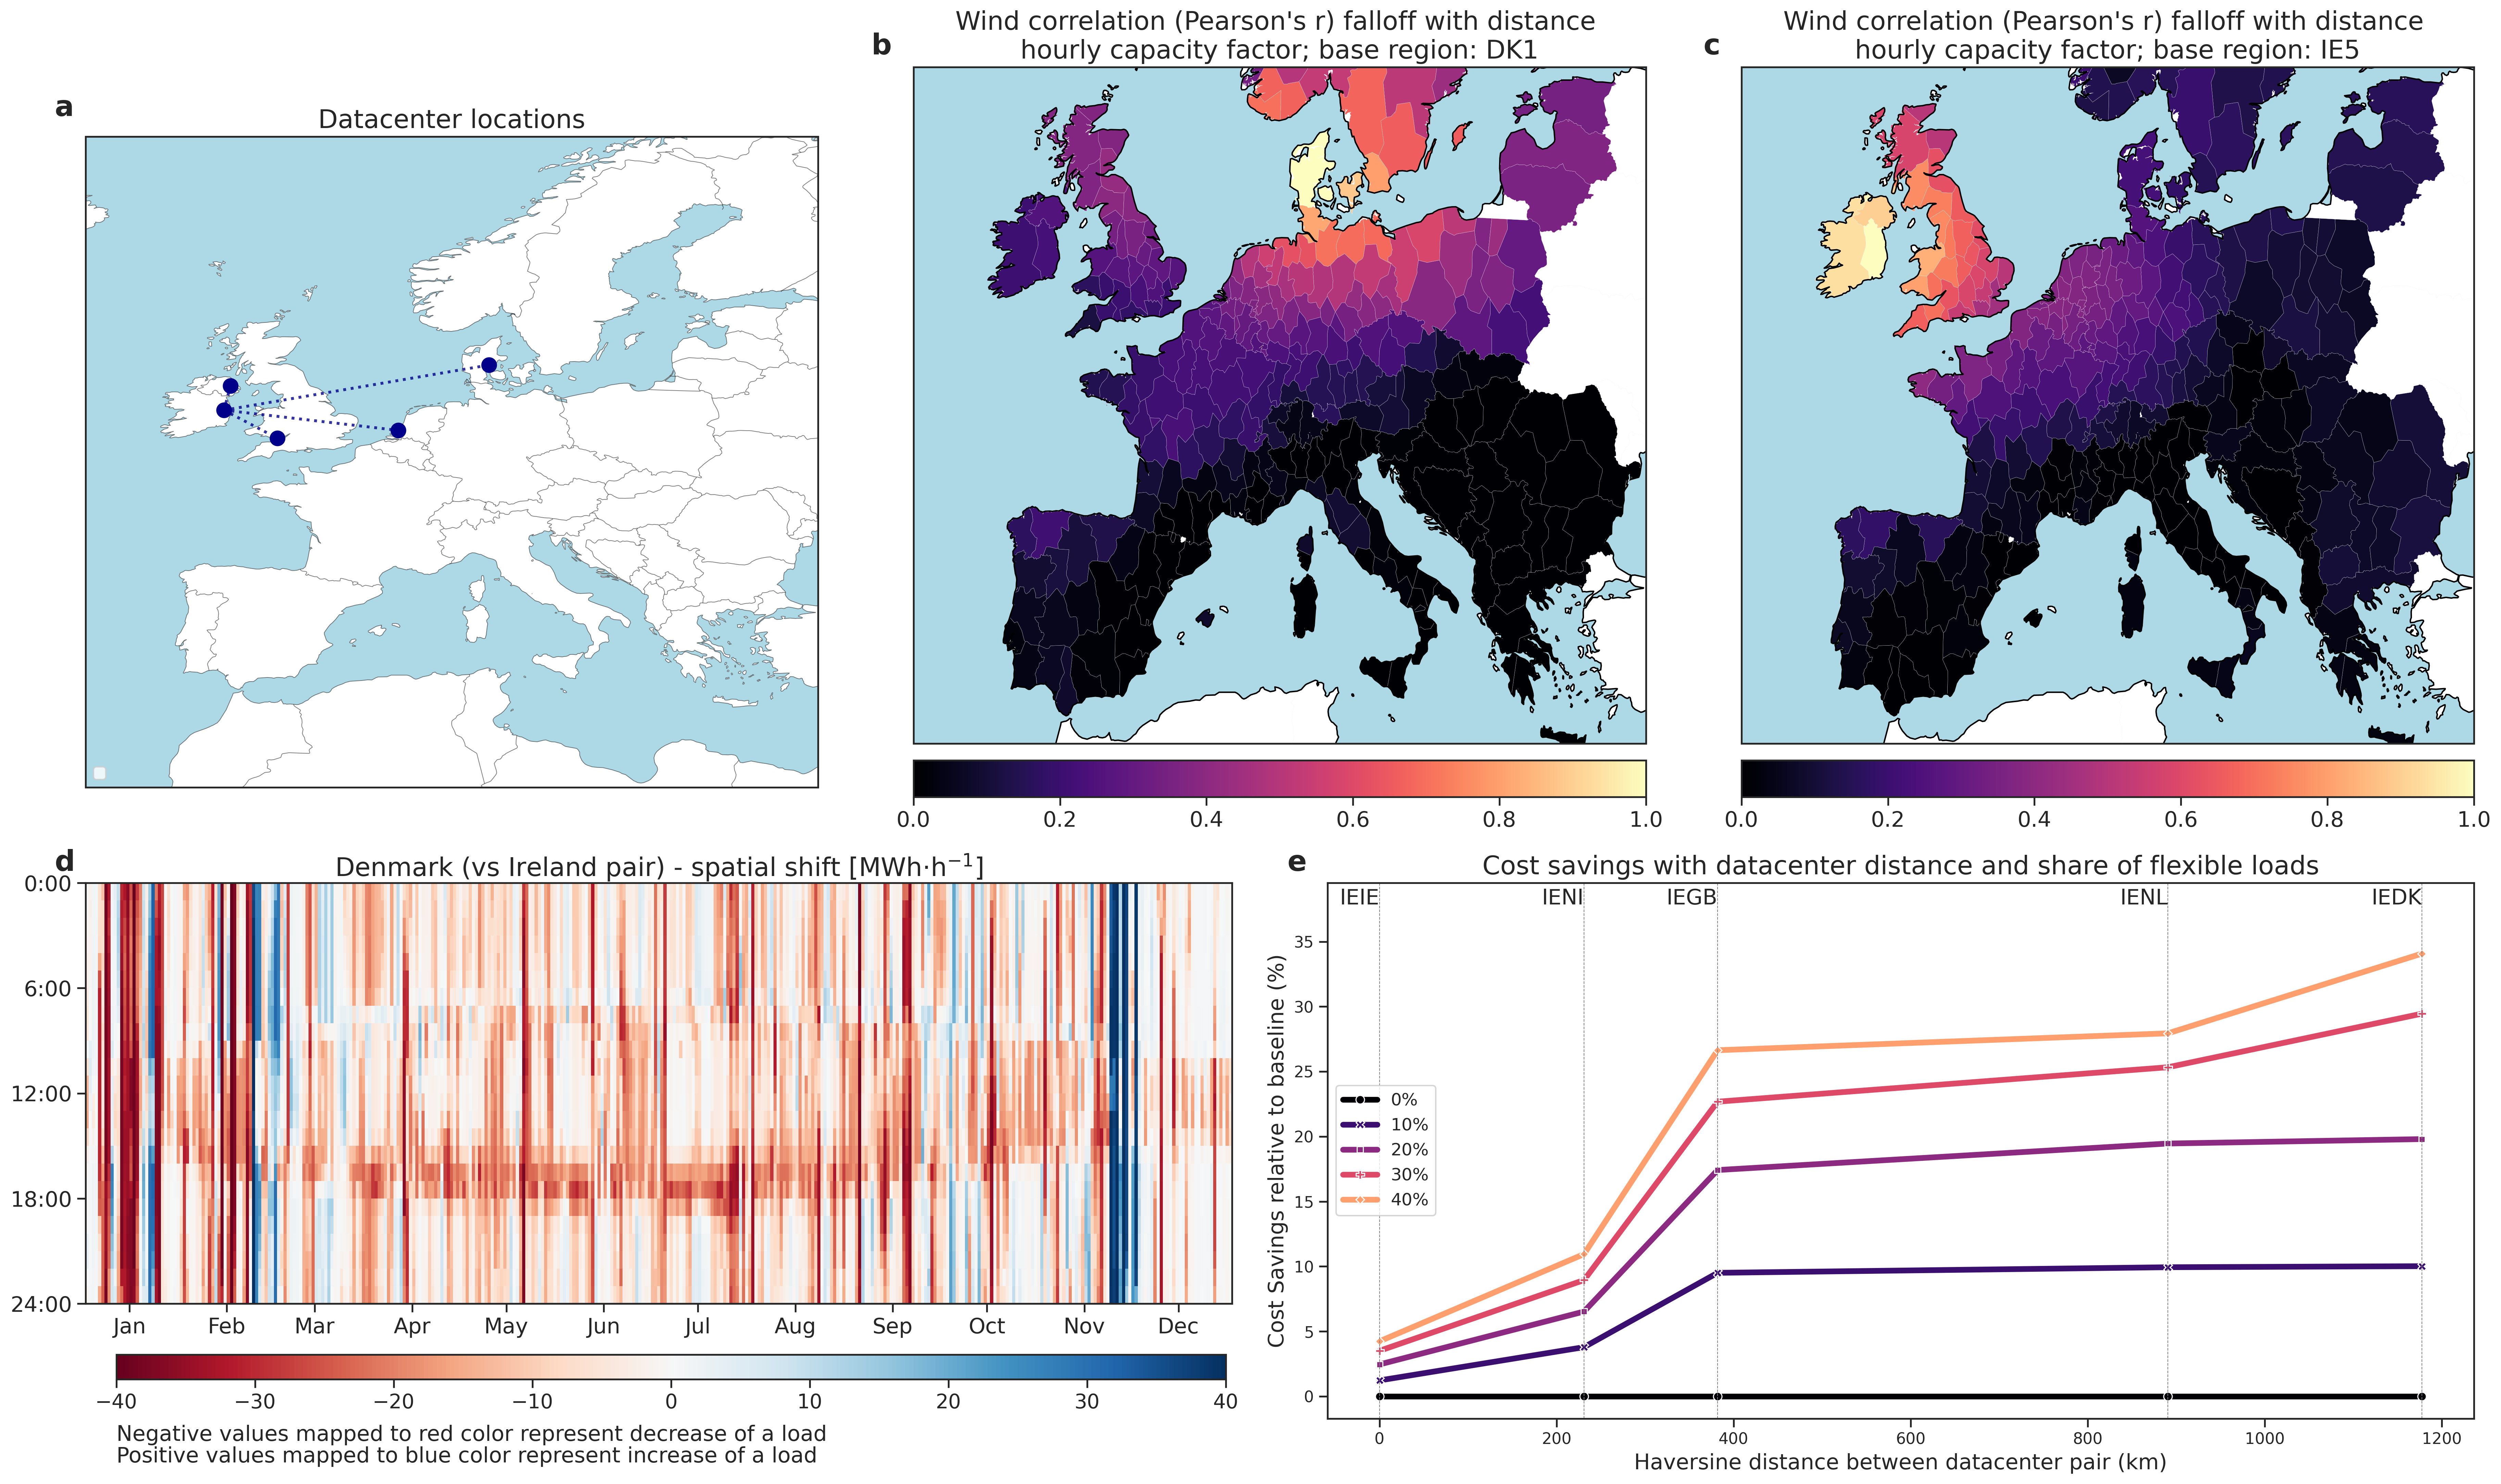
\includegraphics[width=\textwidth]{img/dashboard_2.png}
    \caption{Illustration of the signal 2: low correlation of wind power generation over long distances.
    \textbf{a:} Assumed datacenter locations: pairwise connections across regions with similar quality of renewable resources. Here: Ireland with Northern Ireland, or England, or the Netherlands, or Denmark (-west zone).
    \textbf{b,c:} Peason correlation of hourly capacity factor for onshore wind generation, if Denmark (-west zone, panel b) or selected region of Ireland (panel c) are taken as basis. As a result of different weather conditions, wind feed-in has a noticeable correlation falloff over distances of 300-400 km. Data is simulated using the ERA5 reanalysis dataset for weather year 2013 and aggregated to 256 regions in Europe.
    \textbf{d} Hourly spatial load shifts for the selected scenario and datacenter; here datacenter is located Denmark (and another one is located Ireland). Color mapping represents the quantity of load \enquote{received} from other locations or \enquote{sent} away.
    \textbf{e} Cost savings of 24/7 matching with increasing distance between datacenters. Costs are normalized to the cost level of inflexible load.}
    \label{fig:dashboard2}
\end{figure*}


\subsection{Signal 3: time lag in solar radiation peaks due to Earth's rotation}

Our third step is to isolate the signal associated with the time lag in solar radiation peaks due to Earth's rotation. Consider a case when datacenters are located in Denmark, Greece, and Portugal (Figure \ref{fig:dashboard3}: panel a). In this scenario, Danish datacenter has access to high-quality wind resources, whereas Greek and Portuguese datacenters have access to good solar resources.

The Pearson correlation of the simulated hourly capacity factors for solar photovoltaic generation (Figure \ref{fig:dashboard3}: panels b and c) show that solar generation has good correlation over long distances, in contrast to wind. However, the datacenters in Greece and Portugal are approx. 2700~km apart, which creates potential for the use of spatial flexibility to take advantage of the time lag in solar generation peaks. The difference in solar photovoltaic hourly capacity factors between the two selected locations is shown in Figure \ref{fig:dashboard3}: panel d. The panel illustrates the time lag in solar generation peaks due to Earth's rotation. The peak of solar generation in Portugal is delayed by several hours compared to Greece. For comparison, the difference in wind generation hourly capacity factors between the two selected locations is shown in Figure \ref{fig:dashboard3}: panel e. As expected, low correlation of wind feed-in over long distance results in a stochastic pattern.

Panels f, g and h in Figure \ref{fig:dashboard3} show the cost-optimal portfolio of renewable resources and battery storage for 24/7 matching, cost breakdown, and total annual costs of 24/7 matching strategy as a function of load flexibility. Similar to the previous examples, the cost-optimal portfolio of resources necessary for 24/7 matching and associated costs are reduced with increasing flexible loads, as datacenters can get the most out of the clean energy resources with good quality, as well as take advantage of the time lag in solar generation peaks. In the case of Danish datacenter, benefiting from having partners in solar-rich locations, the costs of 24/7 matching strategy is reduced from 174~\euro/MWh to 157~\euro/MWh with 10\% of flexible loads, and up to 106~\euro/MWh with 40\% of flexible loads.

Finally, Figure \ref{fig:dashboard3}: panels i and j show optimal hourly load shifts for the selected datacenter locations in Greece and Portugal, accordingly. The heatmaps illustrate how spatial flexibility can be used to benefit from the time lag in solar generation peaks. The datacenters in Greece and Portugal receive loads from Denmark between midspring and midfall, with a clear daily pattern caused by the time lag in solar generation peaks. Additionally, the heatmaps show that during the winter months, when solar generation is scarce, both datacenters tend to shift loads to Denmark.

\begin{figure*}
    \centering
    \includegraphics[width=\textwidth]{img/dashboard_3.pdf}
    \caption{Illustration of the signal 3: time lag in solar radiation peaks due to Earth's rotation.
    \textbf{a:} Assumed datacenter locations: Denmark, Portugal, Greece.
    \textbf{b,c:} Peason correlation of hourly capacity factor for solar photovoltaic generation, if selected region of Portugal (panel b) or region of Greece (panel c) is taken as basis. Solar generation remains highly correlated over long distances, in contrast to wind generation.
    \textbf{d:} Difference in solar photovoltaic hourly capacity factors between two selected locations: Greece and Portugal. The two locations are approx. 2700~km apart, which results in a noticeable lag in solar generation peaks due to Earth's rotation.
    \textbf{e:} Difference in wind generation hourly capacity factors between two selected locations: Greece and Portugal. As expected, low correlation of wind feed-in over long distance results in stochastic pattern.
    \textbf{f:} Cost-optimal portfolio of renewable resources and battery storage sufficient for 24/7 matching. Steps on x-axis represent increasing share of flexible load.
    \textbf{g:} Cost breakdown of 24/7 matching strategy.
    \textbf{h:} Total annual costs of 24/7 matching strategy as a function load flexibility. Relative axis is normalized to the costs of inflexible load.
    \textbf{i,j} Hourly spatial load shifts for the selected datacenter locations: Greece (panel i) and Portugal (panel j). Color mapping represents the quantity of load \enquote{received} from other locations or \enquote{sent} away.}
    \label{fig:dashboard3}
\end{figure*}


\subsection{Generalising the results beyond specific load locations}
\label{ssec:section4}

Finally, we aim to generalise the results beyond specific load locations and to provide a more comprehensive understanding of the relationship between load flexibility and the costs of 24/7 CFE matching. 

Consider that datacenters can be located in any of the following eight countries: Denmark, Ireland, the Netherlands, Germany, Latvia, Greece, Portugal, and France. We selected these countries to represent a variety of renewable resources and geographical locations.\footnote{The analysis could be expanded to include additional locations, but the number of combinations would be significantly increased. These locations are a reasonable compromise between generalisation quality and computational demands.} The analysis is carried out by modeling all combinations of three datacenters in the selected countries. With three countries selected from eight, and the order of the countries being irrelevant, there are 56 possible combinations. As a result, the scenario space includes combinations of datacenters with different quality of renewable resources, as well as different distances between them. 
For each combination of datacenters and level of flexibility, we conduct the same analysis as in the previous sections, i.e., the model solution includes information about the cost-optimal portfolio of renewable resources and battery storage for 24/7 matching, procurement policy cost breakdowns, and optimal utilisation of spatial and temporal load flexibility.

The results of the analysis are presented in Figure \ref{fig:flexcost}. The figure shows the relationship between the level of flexibility and the costs of 24/7 matching for all 56 combinations of datacenters. The normalised costs of 24/7 matching lie in a broad range from 240~\euro/MWh to ca. 160~\euro/MWh for inflexible load scenario. The lower bound represents combination Denmark-Greece-Portugal, since these locations share excellent quality of wind and solar resources. The upper bound represents a combination of Germany, Ireland, and Latvia, since none of the three locations have a good solar resource, and only Ireland has a good wind resource.  As a result, 24/7 CFE matching is especially expensive in two out of three locations -- Germany and Latvia. 

Several conclusions can be drawn from the analysis. First, space-time load-shifting flexibility facilitates the efficiency and affordability of 24/7 CFE matching, regardless of the location of the datacenters. Based on specific datacenter locations, the optimal use of space-time flexibility may be influenced by one, or a combination, of the signals discussed above; however, in general, flexibility is beneficial to all locations.

Second, the costs of 24/7 CFE matching are reduced by 1.29$\pm$0.07~\euro/MWh for every additional percentage of flexible load. The low standard error suggests that the relationship is robust across different combinations of datacenters. This finding implies that datacenters can make use of the available flexibility to reduce the costs of 24/7 CFE matching, regardless of which of the three signals is dominant for the specific locations. For example, if renewable energy quality is similar across all locations, and solar PV has a high \gls{lcoe}, the two related signals have little impact on optimal space-time shifting and 24/7 CFE procurement strategy. However, when this occurs, the company operating the datacenters can use all the available load flexibility to \enquote{arbitrage} on low correlation of wind feed-in, and factor this into the procurement strategy.

Third, the overlap between the mean trend and linear regression line suggests that the value of additional flexibility diminishes as the number of flexible loads increases, i.e., the first 10\% of flexible loads can reduce costs more than the next 10\% of flexible loads. The latter is consistent with the observations made in previous sections.


\begin{figure}
    \centering
    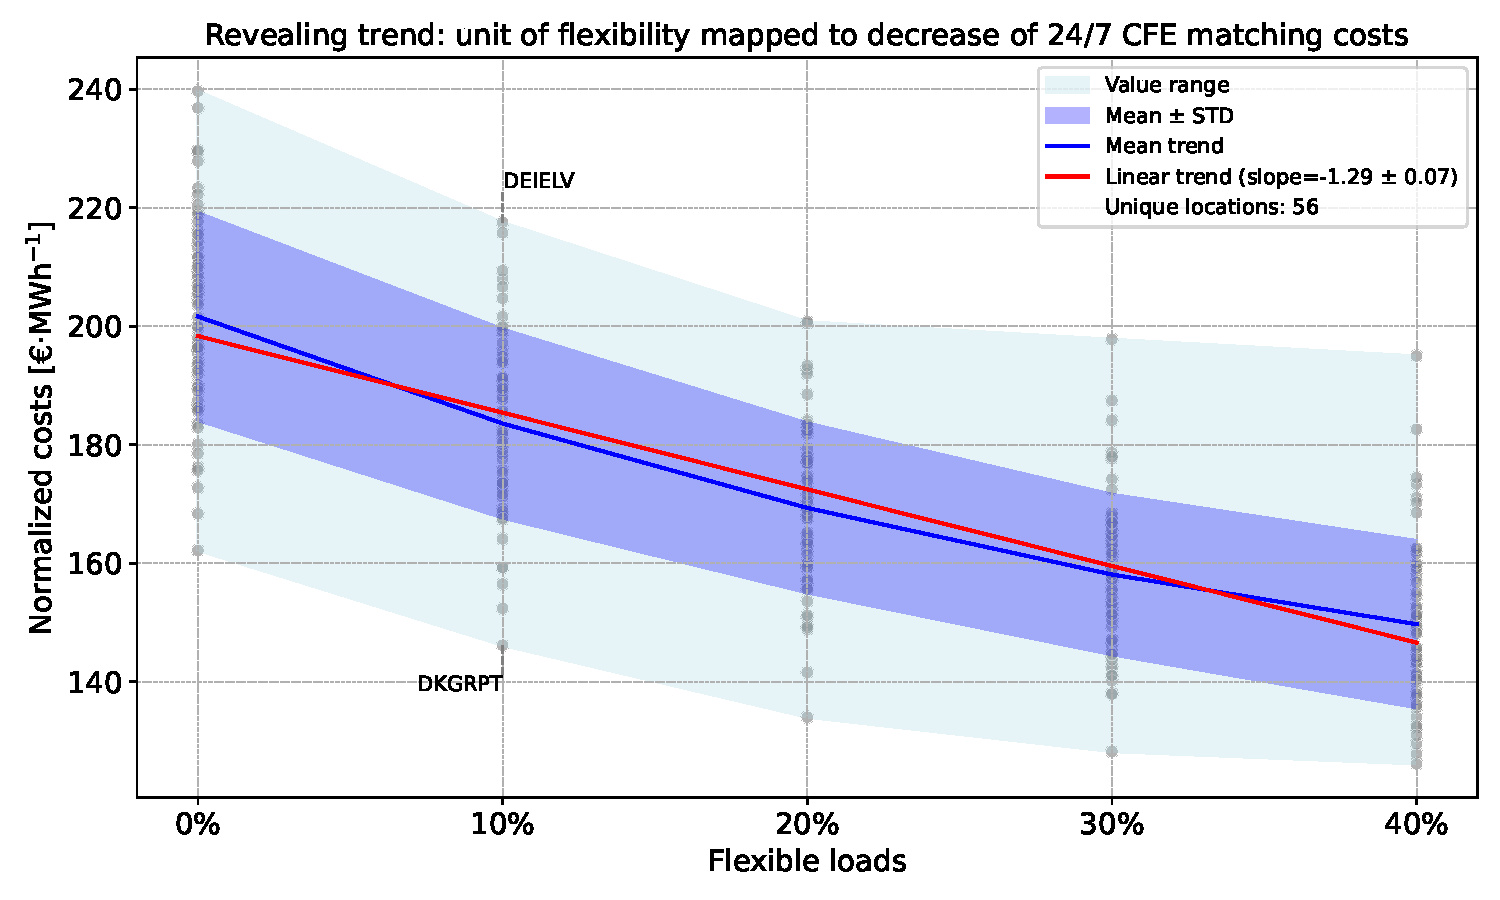
\includegraphics[width=1\columnwidth]{img/flexibility_vs_normalized_costs.pdf}
    \caption{Relationship between the level of flexibility and the costs of 24/7 matching for 56 combinations of datacenter locations. The costs are normalised to the cost level of inflexible load.}
    \label{fig:flexcost}
\end{figure}
